% Options for packages loaded elsewhere
\PassOptionsToPackage{unicode}{hyperref}
\PassOptionsToPackage{hyphens}{url}
\PassOptionsToPackage{dvipsnames,svgnames,x11names}{xcolor}
%
\documentclass[
]{agujournal2019}

\usepackage{amsmath,amssymb}
\usepackage{iftex}
\ifPDFTeX
  \usepackage[T1]{fontenc}
  \usepackage[utf8]{inputenc}
  \usepackage{textcomp} % provide euro and other symbols
\else % if luatex or xetex
  \usepackage{unicode-math}
  \defaultfontfeatures{Scale=MatchLowercase}
  \defaultfontfeatures[\rmfamily]{Ligatures=TeX,Scale=1}
\fi
\usepackage{lmodern}
\ifPDFTeX\else  
    % xetex/luatex font selection
\fi
% Use upquote if available, for straight quotes in verbatim environments
\IfFileExists{upquote.sty}{\usepackage{upquote}}{}
\IfFileExists{microtype.sty}{% use microtype if available
  \usepackage[]{microtype}
  \UseMicrotypeSet[protrusion]{basicmath} % disable protrusion for tt fonts
}{}
\makeatletter
\@ifundefined{KOMAClassName}{% if non-KOMA class
  \IfFileExists{parskip.sty}{%
    \usepackage{parskip}
  }{% else
    \setlength{\parindent}{0pt}
    \setlength{\parskip}{6pt plus 2pt minus 1pt}}
}{% if KOMA class
  \KOMAoptions{parskip=half}}
\makeatother
\usepackage{xcolor}
\setlength{\emergencystretch}{3em} % prevent overfull lines
\setcounter{secnumdepth}{5}
% Make \paragraph and \subparagraph free-standing
\ifx\paragraph\undefined\else
  \let\oldparagraph\paragraph
  \renewcommand{\paragraph}[1]{\oldparagraph{#1}\mbox{}}
\fi
\ifx\subparagraph\undefined\else
  \let\oldsubparagraph\subparagraph
  \renewcommand{\subparagraph}[1]{\oldsubparagraph{#1}\mbox{}}
\fi


\providecommand{\tightlist}{%
  \setlength{\itemsep}{0pt}\setlength{\parskip}{0pt}}\usepackage{longtable,booktabs,array}
\usepackage{calc} % for calculating minipage widths
% Correct order of tables after \paragraph or \subparagraph
\usepackage{etoolbox}
\makeatletter
\patchcmd\longtable{\par}{\if@noskipsec\mbox{}\fi\par}{}{}
\makeatother
% Allow footnotes in longtable head/foot
\IfFileExists{footnotehyper.sty}{\usepackage{footnotehyper}}{\usepackage{footnote}}
\makesavenoteenv{longtable}
\usepackage{graphicx}
\makeatletter
\def\maxwidth{\ifdim\Gin@nat@width>\linewidth\linewidth\else\Gin@nat@width\fi}
\def\maxheight{\ifdim\Gin@nat@height>\textheight\textheight\else\Gin@nat@height\fi}
\makeatother
% Scale images if necessary, so that they will not overflow the page
% margins by default, and it is still possible to overwrite the defaults
% using explicit options in \includegraphics[width, height, ...]{}
\setkeys{Gin}{width=\maxwidth,height=\maxheight,keepaspectratio}
% Set default figure placement to htbp
\makeatletter
\def\fps@figure{htbp}
\makeatother
% definitions for citeproc citations
\NewDocumentCommand\citeproctext{}{}
\NewDocumentCommand\citeproc{mm}{%
  \begingroup\def\citeproctext{#2}\cite{#1}\endgroup}
\makeatletter
 % allow citations to break across lines
 \let\@cite@ofmt\@firstofone
 % avoid brackets around text for \cite:
 \def\@biblabel#1{}
 \def\@cite#1#2{{#1\if@tempswa , #2\fi}}
\makeatother
\newlength{\cslhangindent}
\setlength{\cslhangindent}{1.5em}
\newlength{\csllabelwidth}
\setlength{\csllabelwidth}{3em}
\newenvironment{CSLReferences}[2] % #1 hanging-indent, #2 entry-spacing
 {\begin{list}{}{%
  \setlength{\itemindent}{0pt}
  \setlength{\leftmargin}{0pt}
  \setlength{\parsep}{0pt}
  % turn on hanging indent if param 1 is 1
  \ifodd #1
   \setlength{\leftmargin}{\cslhangindent}
   \setlength{\itemindent}{-1\cslhangindent}
  \fi
  % set entry spacing
  \setlength{\itemsep}{#2\baselineskip}}}
 {\end{list}}
\usepackage{calc}
\newcommand{\CSLBlock}[1]{\hfill\break\parbox[t]{\linewidth}{\strut\ignorespaces#1\strut}}
\newcommand{\CSLLeftMargin}[1]{\parbox[t]{\csllabelwidth}{\strut#1\strut}}
\newcommand{\CSLRightInline}[1]{\parbox[t]{\linewidth - \csllabelwidth}{\strut#1\strut}}
\newcommand{\CSLIndent}[1]{\hspace{\cslhangindent}#1}

\usepackage{booktabs}
\usepackage{longtable}
\usepackage{array}
\usepackage{multirow}
\usepackage{wrapfig}
\usepackage{float}
\usepackage{colortbl}
\usepackage{pdflscape}
\usepackage{tabu}
\usepackage{threeparttable}
\usepackage{threeparttablex}
\usepackage[normalem]{ulem}
\usepackage{makecell}
\usepackage{xcolor}
\usepackage{url} %this package should fix any errors with URLs in refs.
\usepackage{lineno}
\usepackage[inline]{trackchanges} %for better track changes. finalnew option will compile document with changes incorporated.
\usepackage{soul}
\linenumbers
\makeatletter
\@ifpackageloaded{caption}{}{\usepackage{caption}}
\AtBeginDocument{%
\ifdefined\contentsname
  \renewcommand*\contentsname{Table of contents}
\else
  \newcommand\contentsname{Table of contents}
\fi
\ifdefined\listfigurename
  \renewcommand*\listfigurename{List of Figures}
\else
  \newcommand\listfigurename{List of Figures}
\fi
\ifdefined\listtablename
  \renewcommand*\listtablename{List of Tables}
\else
  \newcommand\listtablename{List of Tables}
\fi
\ifdefined\figurename
  \renewcommand*\figurename{Figure}
\else
  \newcommand\figurename{Figure}
\fi
\ifdefined\tablename
  \renewcommand*\tablename{Table}
\else
  \newcommand\tablename{Table}
\fi
}
\@ifpackageloaded{float}{}{\usepackage{float}}
\floatstyle{ruled}
\@ifundefined{c@chapter}{\newfloat{codelisting}{h}{lop}}{\newfloat{codelisting}{h}{lop}[chapter]}
\floatname{codelisting}{Listing}
\newcommand*\listoflistings{\listof{codelisting}{List of Listings}}
\makeatother
\makeatletter
\makeatother
\makeatletter
\@ifpackageloaded{caption}{}{\usepackage{caption}}
\@ifpackageloaded{subcaption}{}{\usepackage{subcaption}}
\makeatother
\ifLuaTeX
  \usepackage{selnolig}  % disable illegal ligatures
\fi
\usepackage{bookmark}

\IfFileExists{xurl.sty}{\usepackage{xurl}}{} % add URL line breaks if available
\urlstyle{same} % disable monospaced font for URLs
\hypersetup{
  pdftitle={Near Infra-Red Spectroscopy Predicts Crude Protein in Hemp Grain},
  pdfauthor={Ryan Crawford; Jamie Crawford; Lawrence B. Smart; Virginia Moore},
  pdfkeywords={Hemp, Grain, Spectroscopy},
  colorlinks=true,
  linkcolor={blue},
  filecolor={Maroon},
  citecolor={Blue},
  urlcolor={Blue},
  pdfcreator={LaTeX via pandoc}}


\draftfalse

\begin{document}
\title{Near Infra-Red Spectroscopy Predicts Crude Protein in Hemp Grain}

\authors{Ryan Crawford\affil{1}, Jamie Crawford\affil{1}, Lawrence B.
Smart\affil{2}, Virginia Moore\affil{3}}
\affiliation{1}{Cornell University, Ithaca, NY, }\affiliation{2}{Cornell
AgriTech, Geneva, NY, }\affiliation{3}{Cornell University, Ithaca, NY, }
\correspondingauthor{Ryan Crawford}{rvc3@cornell.edu}


\begin{abstract}
Lorem ipsum dolor sit amet, consectetur adipiscing elit, sed do eiusmod
tempor incididunt ut labore et dolore magna aliqua. Ut enim ad minim
veniam, quis nostrud exercitation ullamco laboris nisi ut aliquip ex ea
commodo consequat. Duis aute irure dolor in reprehenderit in voluptate
velit esse cillum dolore eu fugiat nulla pariatur. Excepteur sint
occaecat cupidatat non proident, sunt in culpa qui officia deserunt
mollit anim id est laborum.
\end{abstract}

\section*{Plain Language Summary}
Earthquake data for the island of La Palma from the September 2021
eruption is found \ldots{}



\textbf{incomplete: may contain errors, run-ons, half-thoughts, etc.}

\subsection{INTRODUCTION}\label{introduction}

Hemp (Cannabis sativa L.) is an annual crop with potential uses as a
source of food or feed from grain, and bast fiber or hurd from the
stalk. Hemp cultivars are commonly grown for one or both purposes and a
cultivar may be referred to as a grain, fiber, or dual-purpose type.
Because of protein's nutritional importance, the protein content of a
grain crop is an prime consideration for researchers, producers, and
consumers. Whole hemp grain typically contains approximately 20-30\%
protein (Bárta et al., 2024; Ely \& Fike, 2022; \textbf{callaway2004?}).
Crude protein (CP) is often used as a proxy for the direct measurement
of protein concentration and consists of the multiplication of nitrogen
concentration by a conversion factor because measuring nitrogen
concentration is relatively easy and cheap via laboratory assay (Hayes,
2020).

Near-infrared spectroscopy (NIRS) technology is rapid, non-destructive,
and cheap, and consists of the measurement of NIR radiation reflected
from a sample (Roberts et al., 2004). NIR spectra from many samples are
related to laboratory values for components such as moisture, protein,
fat, or fiber (Roberts et al., 2004). NIRS technology has been used
since the 1970's to assess forage CP (Reeves, 2012; Williams, 1975). A
NIRS calibration set often consists of samples from one species grown in
many environments encompassing the range of expected values from the
analyte or analytes (Chadalavada et al., 2022). Partial least squares
regression (PLSR) is a typical method used in the agricultural and food
sciences to relate spectra to analyte (Roberts et al., 2004). PLSR
calculates principal components (PCs) which relate to the dependent
variable and summarize the spectra and uses a subset of PCs in order to
fit the regression model. PLSR is commonly used in spectroscopy because
it tends to work well with highly-correlated spectral data. Typically
the number of principal components is chosen via cross-validation to
avoid overfitting. \textbf{CITES FOR ALL OF THIS}

A NIRS-scanned sample of undamaged grain may used for other purposes or
it may planted as a seed. In wheat and corn, grain protein content has
been shown to be heritable (Geyer et al., 2022; Giancaspro et al.,
2019). This suggests (at least potentially) that NIRS technology could
serve as resource to more rapidly identify high CP hemp germplasm,
enabling the delivery of higher CP hemp grain cultivars faster.

For this study, a benchtop NIR spectrometer was used to develop a model
to predict CP content based on a data set of hemp grain representing
multiple years, locations, and cultivars from grain and dual-purpose
hemp types using PLSR.

\subsection{MATERIALS AND METHODS}\label{materials-and-methods}

\textsubscript{Source:
\href{https://rvcrawford.github.io/glowing-system/index.qmd.html}{Article
Notebook}}

\textsubscript{Source:
\href{https://rvcrawford.github.io/glowing-system/index.qmd.html}{Article
Notebook}}

\subsubsection{Hemp Grain Sample
Background}\label{hemp-grain-sample-background}

Spectral data were obtained from whole (unground) hemp grain samples,
harvested at maturity, collected from 2017 - 2021 from 18 cultivar
trials in New York (NY) (NA samples). Grain samples were obtained by
hand sampling or mechanical harvest and were cleaned of chaff and dried
at 30 C for six days in a forced-air dryer. In total, 38 cultivars were
represented in the data set. Cultivars were grain or dual-purpose types
and included both commercially available and experimental material.

All cultivar trials were planted in randomized complete block design
with each cultivar replicated four times. The 2017 data were comprised
of samples from the same thirteen cultivars sampled from six NY
locations. For those trials, grain was harvested from each plot
individually and aggregated by cultivar within each trial. Four
subsamples were drawn from each aggregated sample and scanned
separately. These spectra were averaged at each 2 nm increment. All
remaining samples from 2018-2021 were collected on a per-plot basis. All
possible cultivars and possible locations were represented in 2017, but
only a selected subset of cultivars and locations were represented in
2018-2021.

\subsubsection{Spectral Data Collection and
Preprocessing}\label{spectral-data-collection-and-preprocessing}

A benchtop NIR spectrometer (FOSS/ NIR FOSS/ NIR Systems model 5000) was
used to obtain the spectra (FOSS North America, Eden Prairie, MN, USA).
Spectra were collected every 2 nm from 1100-2498 nm and the logarithm of
reciprocal reflectance was recorded.

WINISI software version 1.02A (Infrasoft International, Port Matilda,
PA, USA) was used to average the spectra in 2017, as well as to select
samples for laboratory assay. Samples were selected according to their
spectral distance from their nearest neighbor within the calibration
data set with a cutoff of a distance of 0.6 H, where H is approximately
equal to the squared Mahalanobis distance divided by the number of
principal components used in the calculation (Garrido-Varo et al.,
2019). Prior to selection selection, spectra were preprocessed using
SNV-detrend with settings 1,4,4,1 for the derivative, gap, smooth, and
smooth 2 settings respectively.

\subsubsection{Laboratory Validation}\label{laboratory-validation}

Laboratory assays were performed by Dairy One Forage Laboratory (Ithaca,
NY). For those assays, 1mm ground samples were analyzed by combustion
using a CN628 or CN928 Carbon/Nitrogen Determinator. Samples from 2017
were aggregated as described above, but the remaining samples were not
aggregated.

\subsubsection{Model Development}\label{model-development}

Calibration and validations sets were created by dividing the laboratory
CP values into tertiles according to their percent CP in order to ensure
that the range of CP values was present in both calibration and
validation sets. Within each tertile, 75\% of the samples were randomly
assigned to the calibration set and the remaining 25\% were assigned to
the validation set. For each calibration set, models were developed in
caret using PLSR. In fitting the model, the number of principal
components was optimized over au grid search from 1-20. Model
performance was evaluated with 25 iterations of bootstrapping and
minimized root mean squared error (RMSE) in selecting the number of
principal components in the final model .

\textsubscript{Source:
\href{https://rvcrawford.github.io/glowing-system/index.qmd.html}{Article
Notebook}}

Initially a number of common spectral preprocessing methods were tested
by creating 100 calibration and validation sets as described above.
Spectral data from those data sets were transformed by each of the
following methods: 1) first derivative, 2) Savitzky-Golay (SG) using the
first derivative, third order polynomial, and a window of size 5, 3)
gap-segment derivative using the first derivative, a gap of eleven, and
a segment size of 5, 4) standard normal variate (SNV), 4) standard
normal variate following Savitzky-Golay (SNV-SG) (same SG parameters as
above), 5) SNV-detrend with second order polynomial, and 6)
multiplicative scatter correction.

For each of these preprocessing methods, models were fit and predictions
were made on the corresponding validation set (since there were 8
preprocessing methods, 8 separate models were fit for each of the 100
sets. The relationship between the predicted and actual values of the
validation set were calculated via RMSE, R\textsuperscript{2} and Ratio
of Performance to InterQuartile distance (RPIQ), three common model
assessment metrics. Larger R\textsuperscript{2} and RPIQ, and smaller
RMSE values are superior. Analyses of variance (ANOVA) were performed
for each of these metrics in order to compare the preprocessing methods.
For each ANOVA, each data set was considered as a subject and allowing
different variances for each preprocessing method.

Once the most promising preprocessing method was identified, 1000 more
data sets were created and analyzed via that method and performance on
the validation sets was summarized with RMSE, R\textsuperscript{2}, and
RPIQ.

\subsubsection{Additional software used}\label{additional-software-used}

We used R version 4.3.3 (R Core Team, 2024) and the following R
packages: caret v. 6.0.94 (Kuhn \& Max, 2008), data.table v. 1.15.2
(Barrett et al., 2024), emmeans v. 1.10.0 (Lenth, 2024), nlme v. 3.1.163
(J. Pinheiro et al., 2023; J. C. Pinheiro \& Bates, 2000), pls v. 2.8.3
(Liland et al., 2023), prospectr v. 0.2.7 (Stevens \& Ramirez-Lopez,
2024), skimr v. 2.1.5 (Waring et al., 2022), tidymodels v. 1.1.1 (Kuhn
\& Wickham, 2020), tidyverse v. 2.0.0 (Wickham et al., 2019).

\textsubscript{Source:
\href{https://rvcrawford.github.io/glowing-system/index.qmd.html}{Article
Notebook}}

\subsection{RESULTS AND DISCUSSION}\label{results-and-discussion}

\subsubsection{Laboratory assay CP
values}\label{laboratory-assay-cp-values}

Laboratory assay percent CP values are summarized in the following
table. These are similar to the range of CP values observed in the
literature, indicating an reasonable basis for a chemometric model. The
CP values are left-skewed and two thirds of the samples contained more
than 25\% CP.

\begin{longtable}[]{@{}rrrrrrr@{}}

\caption{\label{tbl-lab-protein-vals}Summary of Laboratory Assayed CP
Values (Percent Dry Matter)}

\tabularnewline

\toprule\noalign{}
Mean & Sd & Minimum & First Quartile & Median & Third Quartile &
Maximum \\
\midrule\noalign{}
\endhead
\bottomrule\noalign{}
\endlastfoot
26.1 & 2.5 & 20.8 & 23.9 & 26.4 & 28.2 & 30.8 \\

\end{longtable}

\textsubscript{Source:
\href{https://rvcrawford.github.io/glowing-system/index.qmd.html}{Article
Notebook}}

\subsubsection{Preprocessing methods
comparison}\label{preprocessing-methods-comparison}

\textsubscript{Source:
\href{https://rvcrawford.github.io/glowing-system/index.qmd.html}{Article
Notebook}}

\textsubscript{Source:
\href{https://rvcrawford.github.io/glowing-system/index.qmd.html}{Article
Notebook}}

\textsubscript{Source:
\href{https://rvcrawford.github.io/glowing-system/index.qmd.html}{Article
Notebook}}

\textsubscript{Source:
\href{https://rvcrawford.github.io/glowing-system/index.qmd.html}{Article
Notebook}}

\textsubscript{Source:
\href{https://rvcrawford.github.io/glowing-system/index.qmd.html}{Article
Notebook}}

\textsubscript{Source:
\href{https://rvcrawford.github.io/glowing-system/index.qmd.html}{Article
Notebook}}

All preprocessing methods outperformed raw spectral data
Table~\ref{tbl-preproc}. Averaged together, all preprocessed spectra
were superior to raw spectra, with lower RMSE, and higher
R\textsuperscript{2} and RPIQ values (significant at \(\alpha\) level
\textless0.001). Preprocessing methods had -11.6 \% lower RMSE, and had
3.1\% higher R\textsuperscript{2} 7.4\% higher RPIQ than unprocessed
spectra.

The SNV-SG method had the lowest RMSE, highest R\textsuperscript{2}, and
highest RPIQ averaging over all iterations. SNV-SG RMSE averaged 1.4\%
lower, while R\textsuperscript{2} and RPIQ averaged 0.4\% and 2.4\%
higher respectively than the next best preprocessing method (SG in both
cases), but the difference between the best and second best method by
metric were only statistically significant at \(\alpha\) \textless0.05
for RPIQ. RPIQ was devised to accurately reflect the spread of data in
skewed populations (\textbf{bellon-maurel2010?}) and thus offers a
robust metric for model assessment in this context, where the CP data
are skewed. Therefore the superiority of SNV-SG as measured via RPIQ
made it the best choice for the final model.

\begin{longtable}[]{@{}
  >{\raggedright\arraybackslash}p{(\columnwidth - 6\tabcolsep) * \real{0.5568}}
  >{\raggedright\arraybackslash}p{(\columnwidth - 6\tabcolsep) * \real{0.1477}}
  >{\raggedright\arraybackslash}p{(\columnwidth - 6\tabcolsep) * \real{0.1477}}
  >{\raggedright\arraybackslash}p{(\columnwidth - 6\tabcolsep) * \real{0.1477}}@{}}

\caption{\label{tbl-preproc}Evaluation of Preprocessing Methods by
Metric ± Standard Error}

\tabularnewline

\toprule\noalign{}
\begin{minipage}[b]{\linewidth}\raggedright
Preprocessing Method
\end{minipage} & \begin{minipage}[b]{\linewidth}\raggedright
RMSE
\end{minipage} & \begin{minipage}[b]{\linewidth}\raggedright
\(R^{2}\)
\end{minipage} & \begin{minipage}[b]{\linewidth}\raggedright
RPIQ
\end{minipage} \\
\midrule\noalign{}
\endhead
\bottomrule\noalign{}
\endlastfoot
Standard Normal Variate following Savitzky-Golay & 1.02 ± 0.012 & 0.84 ±
0.004 & 3.97 ± 0.076 \\
Savitzky-Golay & 1.03 ± 0.012 & 0.83 ± 0.004 & 3.88 ± 0.072 \\
First Derivative & 1.07 ± 0.013 & 0.82 ± 0.004 & 3.77 ± 0.075 \\
Standard Normal Variate & 1.12 ± 0.016 & 0.80 ± 0.005 & 3.61 ± 0.081 \\
Gap-segment Derivative & 1.12 ± 0.018 & 0.81 ± 0.006 & 3.60 ± 0.086 \\
Standard Normal Variate-Detrend & 1.13 ± 0.015 & 0.80 ± 0.005 & 3.55 ±
0.079 \\
Multiplicative Scatter Correction & 1.17 ± 0.016 & 0.79 ± 0.006 & 3.47 ±
0.080 \\
Raw Spectra & 1.22 ± 0.044 & 0.79 ± 0.009 & 3.42 ± 0.105 \\

\end{longtable}

\textsubscript{Source:
\href{https://rvcrawford.github.io/glowing-system/index.qmd.html}{Article
Notebook}}

SNV and SNV-detrend correct light scatter. SG is a smoothing filter that
regresses on the signal over a series of windows. Derivatives remove
noise, but not necessarily light scattering. \textbf{cite}

\textbf{cite:} Barnes RJ, Dhanoa MS, Lister SJ. 1989. Standard normal
variate transformation and de-trending of near-infrared diffuse
reflectance spectra. Applied spectroscopy, 43(5): 772-777.

The preprocessing methods examined represent a portion of those
available. As well, preprocessing methods tend to have a number of
user-adjustable parameters whose various permutations were not tested.
This subset of preprocessing methods and parameters nonetheless
contained substantial variations in model quality, demonstrating the
importance of the selection of an appropriate preprocessing method.

\subsubsection{Final model development and
summary}\label{final-model-development-and-summary}

\textsubscript{Source:
\href{https://rvcrawford.github.io/glowing-system/index.qmd.html}{Article
Notebook}}

The model improved most rapidly as the number of principal components
increased from 1 to 7, with the inclusion of each additional PC being
associated with a decrease in RMSE of 5-12\% . From 8 to 12 PCs, model
performance continued to improve, although gains were more modest
(decrease in RMSE of 0.7-3\%). With 13 or more PCs, performance gains
were minimal and the relative ranks of the models tended to be stable
Figure~\ref{fig-model-calibration}.

\phantomsection\label{cell-fig-model-calibration}
\begin{figure}[H]

\centering{

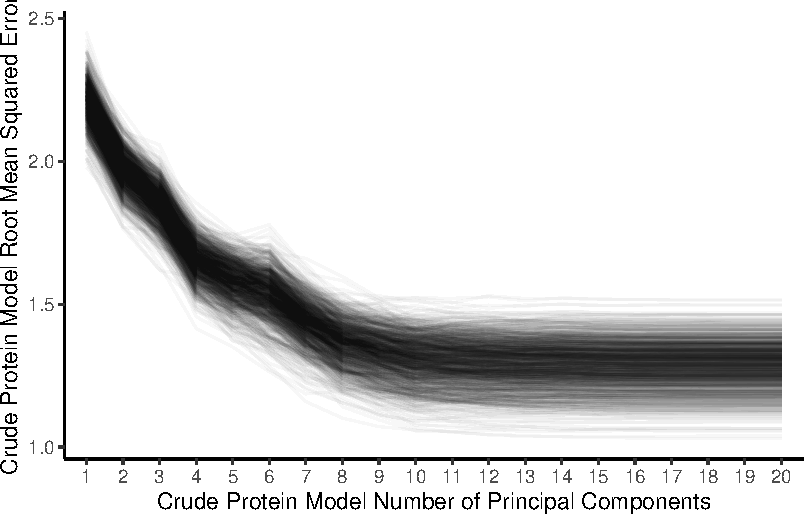
\includegraphics{index_files/figure-pdf/fig-model-calibration-1.pdf}

}

\caption{\label{fig-model-calibration}Decreasing RMSE with increasing
number of PCs}

\end{figure}%

\textsubscript{Source:
\href{https://rvcrawford.github.io/glowing-system/index.qmd.html}{Article
Notebook}}

\textsubscript{Source:
\href{https://rvcrawford.github.io/glowing-system/index.qmd.html}{Article
Notebook}}

Final model performance was similar, but not identical to, that obtained
during the initial comparison of preprocessing methods. The final
models' mean RMSE was 1.03, R\textsuperscript{2} was 0.83, and RPIQ was
3.89 (all calculated on the test sets). Despite the generally good model
performance, a subset of poor models can be seen. For example,
Figure~\ref{fig-final-metric-boxplot} shows twenty-one models with
R\textsuperscript{2} below 0.7. \textbf{more comment on poor models?}

\textsubscript{Source:
\href{https://rvcrawford.github.io/glowing-system/index.qmd.html}{Article
Notebook}}

\phantomsection\label{cell-fig-final-metric-boxplot}
\begin{figure}[H]

\centering{

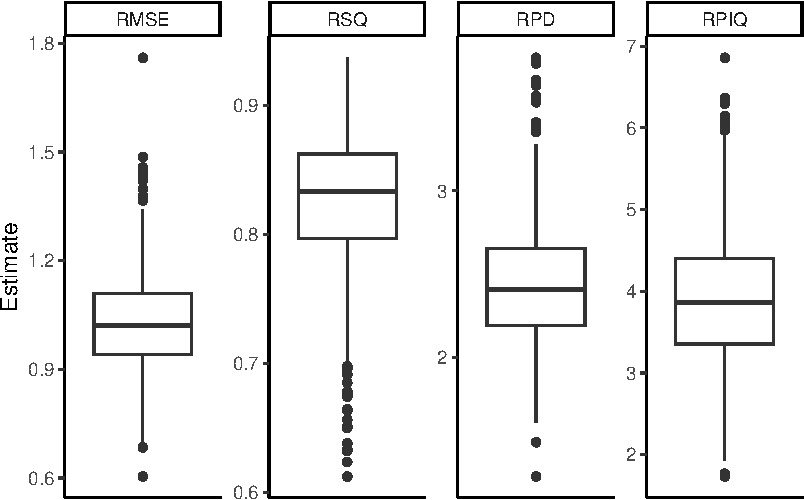
\includegraphics{index_files/figure-pdf/fig-final-metric-boxplot-1.pdf}

}

\caption{\label{fig-final-metric-boxplot}Final model validation set
performance (1000 iterations)}

\end{figure}%

\textsubscript{Source:
\href{https://rvcrawford.github.io/glowing-system/index.qmd.html}{Article
Notebook}}

\textsubscript{Source:
\href{https://rvcrawford.github.io/glowing-system/index.qmd.html}{Article
Notebook}}

\textsubscript{Source:
\href{https://rvcrawford.github.io/glowing-system/index.qmd.html}{Article
Notebook}}

\begin{verbatim}

Call:
lm(formula = difference ~ adj_cp, data = temp_dat)

Residuals:
     Min       1Q   Median       3Q      Max 
-2.51794 -0.58132  0.06936  0.50754  2.74745 

Coefficients:
            Estimate Std. Error t value Pr(>|t|)    
(Intercept)  0.80412    0.17827   4.511 1.31e-05 ***
adj_cp      -0.15334    0.03051  -5.026 1.44e-06 ***
---
Signif. codes:  0 '***' 0.001 '**' 0.01 '*' 0.05 '.' 0.1 ' ' 1

Residual standard error: 0.9138 on 147 degrees of freedom
Multiple R-squared:  0.1466,    Adjusted R-squared:  0.1408 
F-statistic: 25.26 on 1 and 147 DF,  p-value: 1.438e-06
\end{verbatim}

\begin{verbatim}
     ith_in_data_set      preds crude_protein   cutpoints plot_order
               <int>      <num>         <num>      <fctr>      <int>
  1:              50  0.8041160          20.8 (20.8,24.1]          1
  2:              42  0.7274479          21.3 (20.8,24.1]          2
  3:              52  0.6967806          21.5 (20.8,24.1]          3
  4:              83  0.6814470          21.6 (20.8,24.1]          4
  5:              85  0.6814470          21.6 (20.8,24.1]          5
 ---                                                                
145:              12 -0.6219116          30.1 (27.5,30.8]        145
146:              55 -0.6219116          30.1 (27.5,30.8]        146
147:             117 -0.6372452          30.2 (27.5,30.8]        147
148:              63 -0.6679125          30.4 (27.5,30.8]        148
149:             112 -0.7292470          30.8 (27.5,30.8]        149
\end{verbatim}

\textsubscript{Source:
\href{https://rvcrawford.github.io/glowing-system/index.qmd.html}{Article
Notebook}}

Finally, the pattern of errors was examined on a per-sample basis.
Figure~\ref{fig-validation_set_performance}

\phantomsection\label{cell-fig-validation_set_performance}
\begin{figure}[H]

\centering{

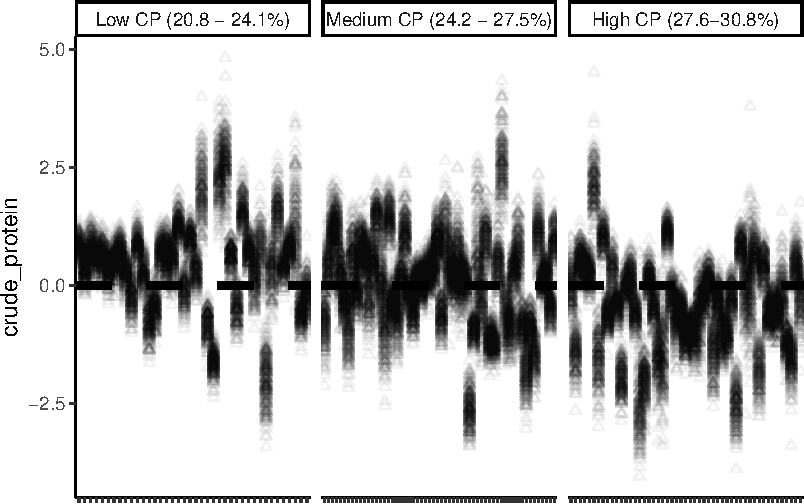
\includegraphics{index_files/figure-pdf/fig-validation_set_performance-1.pdf}

}

\caption{\label{fig-validation_set_performance}Test set prediction
errors on a per-sample basis. Actual sample value set to 0, and samples
ranked from least to greatest.}

\end{figure}%

\textsubscript{Source:
\href{https://rvcrawford.github.io/glowing-system/index.qmd.html}{Article
Notebook}}

Errors tend to be lower at higher levels of actual CP

This study is limited in that it represents the creation of one model
based upon spectra collected from one machine. NIRS calibrations can be
unique to a particular machine, even if the machines compared are of the
same model (\textbf{Reeves\_2012?}) . As well, the calibration and
validation sets are relatively small.

This research showed the promise of the use of NIRS in order to make
predictions concerning \%CP in hemp grain using PLS. Promising
preprocessing methods were identified and a model was validated. Further
research could refine the model by including more samples or by
examining other predictive methods.

\subsection{ACKNOWLEDGMENTS}\label{acknowledgments}

\subsection{SUPPLEMENTAL MATERIAL}\label{supplemental-material}

\textsubscript{Source:
\href{https://rvcrawford.github.io/glowing-system/index.qmd.html}{Article
Notebook}}

\begin{longtable}[]{@{}lrrrrrr@{}}

\caption{\label{tbl-hemp_provenance}Tally of hemp cultivars and
locations. Private cultivars are labeled ``cultivar1'', ``cultivar2'',
etc.}

\tabularnewline

\toprule\noalign{}
cultivar2 & chazy & freeville & geneva & ithaca & willsboro & Total \\
\midrule\noalign{}
\endhead
\bottomrule\noalign{}
\endlastfoot
altair & & & & 1 & & 1 \\
anka & & 1 & 3 & 5 & 2 & 11 \\
bialobrzeskie & & 1 & 3 & 4 & 1 & 9 \\
canda & & 1 & 1 & 1 & & 3 \\
cfx-1 & & 1 & 2 & 5 & & 8 \\
cfx-2 & & 1 & 2 & 4 & & 7 \\
crs-1 & 1 & 1 & 2 & 5 & & 9 \\
cultivar1 & & 1 & & & & 1 \\
cultivar2 & & & & 1 & & 1 \\
cultivar3 & & & & 1 & & 1 \\
cultivar4 & & & & 1 & & 1 \\
earlina 8 & & & 1 & & & 1 \\
experimental1 & & & & 1 & & 1 \\
experimental2 & & & & 1 & & 1 \\
felina 32 & & 1 & 2 & 3 & & 6 \\
futura 75 & & 1 & 3 & 4 & & 8 \\
grandi & & 3 & 3 & 4 & & 10 \\
h-51 & & & 1 & 2 & & 3 \\
han-fn-h & & & & 1 & & 1 \\
han-nw & & & & 1 & & 1 \\
helena & & 1 & & & & 1 \\
henola & & & & 2 & & 2 \\
hlesia & & & & 3 & & 3 \\
hliana & & & 1 & 1 & & 2 \\
joey & & 1 & 1 & 1 & & 3 \\
katani & & 2 & 3 & 4 & & 9 \\
nebraska (feral) & 1 & & & 1 & & 2 \\
pewter river & & 1 & & & & 1 \\
picolo & & 1 & 2 & 5 & & 8 \\
portugal & & & 1 & & & 1 \\
rocky hemp & & & 1 & & & 1 \\
sterling gold & & & 1 & & & 1 \\
swift & 1 & 1 & & 1 & & 3 \\
tygra & & 1 & 3 & 4 & & 8 \\
uso-31 & 2 & 1 & 2 & 4 & & 9 \\
wojko & & 1 & 3 & 4 & & 8 \\
x-59 & & 2 & & 1 & & 3 \\
Total & 5 & 24 & 41 & 76 & 3 & 149 \\

\end{longtable}

\textsubscript{Source:
\href{https://rvcrawford.github.io/glowing-system/index.qmd.html}{Article
Notebook}}

\subsection{OPTIONAL SECTIONS}\label{optional-sections}

\subsection{REFERENCES}\label{references}

\subsection{FIGURES AND TABLES}\label{figures-and-tables}

\textsubscript{Source:
\href{https://rvcrawford.github.io/glowing-system/index.qmd.html}{Article
Notebook}}

\phantomsection\label{cell-fig-timeline}
\begin{figure}[H]

\centering{

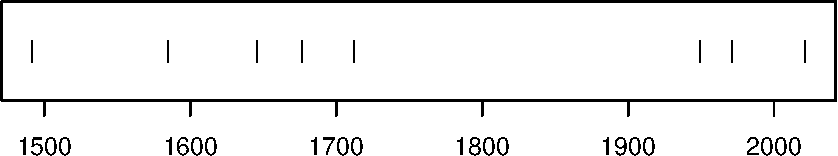
\includegraphics{index_files/figure-pdf/fig-timeline-1.pdf}

}

\caption{\label{fig-timeline}Timeline of recent earthquakes on La Palma}

\end{figure}%

\textsubscript{Source:
\href{https://rvcrawford.github.io/glowing-system/index.qmd.html}{Article
Notebook}}

\textsubscript{Source:
\href{https://rvcrawford.github.io/glowing-system/index.qmd.html}{Article
Notebook}}

Based on data up to and including 1971, eruptions on La Palma happen
every 79.8 years on average.

Studies of the magma systems feeding the volcano, such as
(\textbf{marrero2019?}), have proposed that there are two main magma
reservoirs feeding the Cumbre Vieja volcano; one in the mantle (30-40km
depth) which charges and in turn feeds a shallower crustal reservoir
(10-20km depth).

Eight eruptions have been recorded since the late 1400s
(Figure~\ref{fig-timeline}).

Data and methods are discussed in Section~\ref{sec-data-methods}.

Let \(x\) denote the number of eruptions in a year. Then, \(x\) can be
modeled by a Poisson distribution

\begin{equation}\phantomsection\label{eq-poisson}{
p(x) = \frac{e^{-\lambda} \lambda^{x}}{x !}
}\end{equation}

where \(\lambda\) is the rate of eruptions per year. Using
Equation~\ref{eq-poisson}, the probability of an eruption in the next
\(t\) years can be calculated.

\begin{longtable}[]{@{}ll@{}}
\caption{Recent historic eruptions on La
Palma}\label{tbl-history}\tabularnewline
\toprule\noalign{}
Name & Year \\
\midrule\noalign{}
\endfirsthead
\toprule\noalign{}
Name & Year \\
\midrule\noalign{}
\endhead
\bottomrule\noalign{}
\endlastfoot
Current & 2021 \\
Teneguía & 1971 \\
Nambroque & 1949 \\
El Charco & 1712 \\
Volcán San Antonio & 1677 \\
Volcán San Martin & 1646 \\
Tajuya near El Paso & 1585 \\
Montaña Quemada & 1492 \\
\end{longtable}

Table~\ref{tbl-history} summarises the eruptions recorded since the
colonization of the islands by Europeans in the late 1400s.

\begin{figure}

\centering{

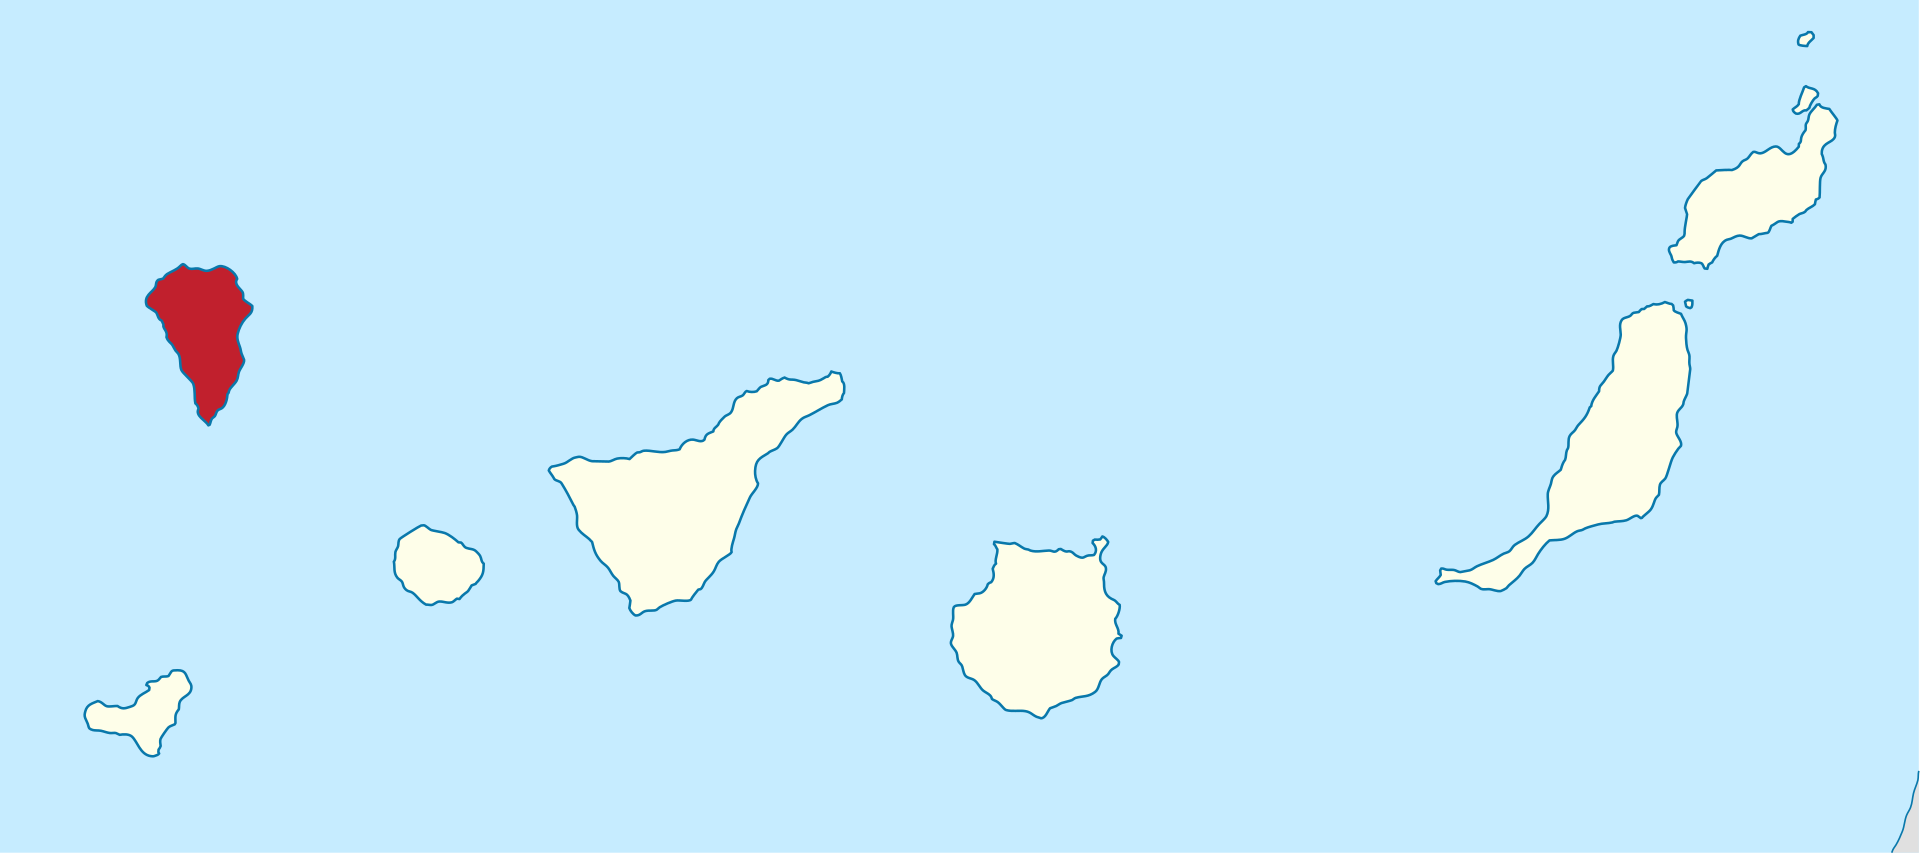
\includegraphics{images/la-palma-map.png}

}

\caption{\label{fig-map}Map of La Palma}

\end{figure}%

La Palma is one of the west most islands in the Volcanic Archipelago of
the Canary Islands (Figure~\ref{fig-map}).

\begin{figure}[H]

\centering{

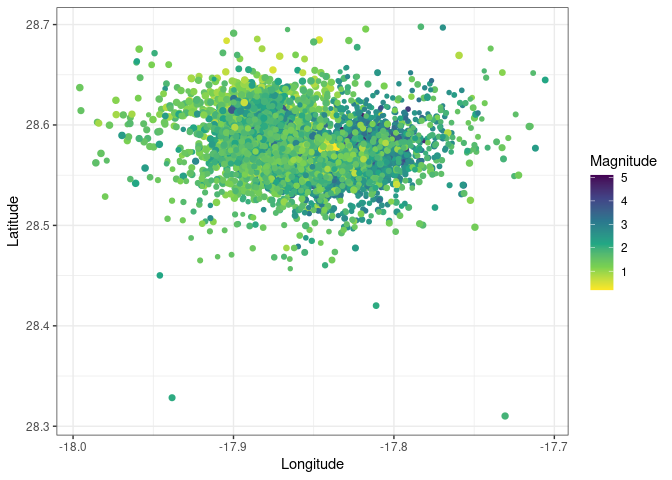
\includegraphics{index_files/figure-latex/notebooks-explore-earthquakes-fig-spatial-plot-output-1.png}

}

\caption{\label{fig-spatial-plot}Locations of earthquakes on La Palma
since 2017}

\end{figure}%

\textsubscript{Source:
\href{https://rvcrawford.github.io/glowing-system/notebooks/explore-earthquakes-preview.html\#cell-fig-spatial-plot}{Explore
Earthquakes}}

Figure~\ref{fig-spatial-plot} shows the location of recent Earthquakes
on La Palma.

\subsection{Data \& Methods}\label{sec-data-methods}

\subsection{Conclusion}\label{conclusion}

\subsection*{References}\label{references-1}
\addcontentsline{toc}{subsection}{References}

\phantomsection\label{refs}
\begin{CSLReferences}{1}{0}
\vspace{1em}

\bibitem[\citeproctext]{ref-datatable}
Barrett, T., Dowle, M., Srinivasan, A., Gorecki, J., Chirico, M., \&
Hocking, T. (2024). \emph{{data.table}: Extension of
{``{data.frame}''}}. \url{https://CRAN.R-project.org/package=data.table}

\bibitem[\citeproctext]{ref-barta_proteomic_2024}
Bárta, J., Roudnický, P., Jarošová, M., Zdráhal, Z., Stupková, A.,
Bártová, V., Krejčová, Z., Kyselka, J., Filip, V., Říha, V., Lorenc, F.,
Bedrníček, J., \& Smetana, P. (2024). Proteomic {Profiles} of {Whole}
{Seeds}, {Hulls}, and {Dehulled} {Seeds} of {Two} {Industrial} {Hemp}
({Cannabis} sativa {L}.) {Cultivars}. \emph{Plants}, \emph{13}(1), 111.
\url{https://doi.org/10.3390/plants13010111}

\bibitem[\citeproctext]{ref-chadalavada_nir_2022}
Chadalavada, K., Anbazhagan, K., Ndour, A., Choudhary, S., Palmer, W.,
Flynn, J. R., Mallayee, S., Pothu, S., Prasad, K. V. S. V.,
Varijakshapanikar, P., Jones, C. S., \& Kholová, J. (2022). {NIR}
{Instruments} and {Prediction} {Methods} for {Rapid} {Access} to {Grain}
{Protein} {Content} in {Multiple} {Cereals}. \emph{Sensors (Basel,
Switzerland)}, \emph{22}(10). \url{https://doi.org/10.3390/s22103710}

\bibitem[\citeproctext]{ref-ely_industrial_2022}
Ely, K., \& Fike, J. (2022). Industrial {Hemp} and {Hemp} {Byproducts}
as {Sustainable} {Feedstuffs} in {Livestock} {Diets}. In D. C. Agrawal,
R. Kumar, \& M. Dhanasekaran (Eds.), \emph{Cannabis/{Hemp} for
{Sustainable} {Agriculture} and {Materials}} (pp. 145--162). Springer.
\url{https://doi.org/10.1007/978-981-16-8778-5_6}

\bibitem[\citeproctext]{ref-garrido-varo_note_2019}
Garrido-Varo, A., Garcia-Olmo, J., \& Fearn, T. (2019). A note on
{Mahalanobis} and related distance measures in {WinISI} and {The}
{Unscrambler}. \emph{Journal of Near Infrared Spectroscopy},
\emph{27}(4), 253--258. \url{https://doi.org/10.1177/0967033519848296}

\bibitem[\citeproctext]{ref-geyer_genetics_2022}
Geyer, M., Mohler, V., \& Hartl, L. (2022). Genetics of the {Inverse}
{Relationship} between {Grain} {Yield} and {Grain} {Protein} {Content}
in {Common} {Wheat}. \emph{Plants}, \emph{11}(16), 2146.
\url{https://doi.org/10.3390/plants11162146}

\bibitem[\citeproctext]{ref-giancaspro_genetic_2019}
Giancaspro, A., Giove, S. L., Blanco, A., \& Gadaleta, A. (2019).
Genetic {Variation} for {Protein} {Content} and {Yield}-{Related}
{Traits} in a {Durum} {Population} {Derived} {From} an
{Inter}-{Specific} {Cross} {Between} {Hexaploid} and {Tetraploid}
{Wheat} {Cultivars}. \emph{Frontiers in Plant Science}, \emph{10}.
\url{https://doi.org/10.3389/fpls.2019.01509}

\bibitem[\citeproctext]{ref-hayes_measuring_2020}
Hayes, M. (2020). Measuring {Protein} {Content} in {Food}: {An}
{Overview} of {Methods}. \emph{Foods}, \emph{9}(10), 1340.
\url{https://doi.org/10.3390/foods9101340}

\bibitem[\citeproctext]{ref-tidymodels}
Kuhn, M., \& Wickham, H. (2020). \emph{{Tidymodels}: A collection of
packages for modeling and machine learning using tidyverse principles.}
\url{https://www.tidymodels.org}

\bibitem[\citeproctext]{ref-caret}
Kuhn, \& Max. (2008). Building predictive models in r using the caret
package. \emph{Journal of Statistical Software}, \emph{28}(5), 1--26.
\url{https://doi.org/10.18637/jss.v028.i05}

\bibitem[\citeproctext]{ref-emmeans}
Lenth, R. V. (2024). \emph{{emmeans}: Estimated marginal means, aka
least-squares means}. \url{https://CRAN.R-project.org/package=emmeans}

\bibitem[\citeproctext]{ref-pls}
Liland, K. H., Mevik, B.-H., \& Wehrens, R. (2023). \emph{{pls}: Partial
least squares and principal component regression}.
\url{https://CRAN.R-project.org/package=pls}

\bibitem[\citeproctext]{ref-nlme2000}
Pinheiro, J. C., \& Bates, D. M. (2000). \emph{Mixed-effects models in s
and s-PLUS}. Springer. \url{https://doi.org/10.1007/b98882}

\bibitem[\citeproctext]{ref-nlme2023}
Pinheiro, J., Bates, D., \& R Core Team. (2023). \emph{{nlme}: Linear
and nonlinear mixed effects models}.
\url{https://CRAN.R-project.org/package=nlme}

\bibitem[\citeproctext]{ref-base}
R Core Team. (2024). \emph{{R}: A language and environment for
statistical computing}. R Foundation for Statistical Computing.
\url{https://www.R-project.org/}

\bibitem[\citeproctext]{ref-reeves_potential_2012}
Reeves, J. B. (2012). Potential of {Near}- and {Mid}-infrared
{Spectroscopy} in {Biofuel} {Production}. \emph{Communications in Soil
Science and Plant Analysis}, \emph{43}(1-2), 478--495.
\url{https://doi.org/10.1080/00103624.2012.641844}

\bibitem[\citeproctext]{ref-roberts_near-infrared_2004}
Roberts, C. A., Workman, J., \& Reeves, J. B. (2004).
\emph{Near-infrared spectroscopy in agriculture}. American Society of
Agronomy.

\bibitem[\citeproctext]{ref-prospectr}
Stevens, A., \& Ramirez-Lopez, L. (2024). \emph{An introduction to the
prospectr package}.

\bibitem[\citeproctext]{ref-skimr}
Waring, E., Quinn, M., McNamara, A., Arino de la Rubia, E., Zhu, H., \&
Ellis, S. (2022). \emph{{skimr}: Compact and flexible summaries of
data}. \url{https://CRAN.R-project.org/package=skimr}

\bibitem[\citeproctext]{ref-tidyverse}
Wickham, H., Averick, M., Bryan, J., Chang, W., McGowan, L. D.,
François, R., Grolemund, G., Hayes, A., Henry, L., Hester, J., Kuhn, M.,
Pedersen, T. L., Miller, E., Bache, S. M., Müller, K., Ooms, J.,
Robinson, D., Seidel, D. P., Spinu, V., \ldots{} Yutani, H. (2019).
Welcome to the {tidyverse}. \emph{Journal of Open Source Software},
\emph{4}(43), 1686. \url{https://doi.org/10.21105/joss.01686}

\bibitem[\citeproctext]{ref-williams_application_1975}
Williams, P. C. (1975). Application of near infrared reflectance
spectroscopy to analysis of cereal grains and oilseeds. \emph{Cereal
Chemistry}, \emph{52}(4 p.561-576), 576--561.

\end{CSLReferences}



\end{document}
